\chapter{System Overview}

\section{Model Architecture}\label{sec:model_arch}
\subsection{hgru4rec}
In section~\ref{sec:hgru4rec} we introduced the model architecture for hgru4rec.
This work proposes and improvement of this model by using the model introduced in~\ref{sec:meta_prod2vec}.
As mentioned before hgru4rec uses a one-hot encoding of items as the input, as seen in equation~\ref{eq:hgru4rec_session}.
We propose to use pre-computed embeddings resulting from Meta-Prod2Vec as a replacement for the one-hot encodings.
Therefore the model architecture is not different from the one seen in figure~\ref{fig:hgru4rec}.
Meta-Prod2Vec is implemented and trained independently of the session-based model.
After training Meta-Prod2Vec, the product embeddings are extracted and saved to a key-value store.
Afterwards hgru4rec can access this key-value store during training and inference such that the model can consume the product embeddings instead of the one-hot vectors.
Further we will test hgru4rec without the user layer, to verify the improvement recorded by the authors of~\cite{hierarchical} using our dataset.
Therefore this work investigates 4 different architectures documented in~\ref{tab:model_archs}.
\begin{table}[t]
    \centering
    \begin{tabular}{llll}\toprule
        \textbf{Model Name} & \textbf{One-Hot} & \textbf{Embedding} & \textbf{User Layer} \\ \midrule
        OnlySessionOneHot & x & - & - \\
        OnlySessionEmbedding & - & x & - \\
        WithUserOneHot & x & - & x \\
        WithUserEmbedding & - & x & x \\ \bottomrule
    \end{tabular}
    \caption{Model Architectures}
    \label{tab:model_archs}
\end{table}
\paragraph{Model training}
After testing different optimizers the Adam optimizer performed best, therefore we used this for training the hierarchical RNN.
The model was trained until there was no more improvement in the validation metric.
The mean reciprocal rank (MRR) at 10 was used as the validation metric.
The reciprocal rank is defined in equation~\ref{eq:reciprocal_rank}

\begin{equation}\label{eq:reciprocal_rank}
    \text{RR} = 
    \begin{cases}
        \frac{1}{\text{rank}(\text{label})} & \text{if label } \in \text{predictions} \\
        0 & \text{otherwise}
    \end{cases}
\end{equation}

Where predictions are the Top 10 predictions returned by the model and $\text{rank}(x)$ is the position of $x$ in those predictions.
The MRR is the mean of the RR over all datapoints.

\subsection{Meta-Prod2Vec}
In section~\ref{sec:meta_prod2vec} we introduced the model architecture for Meta-Prod2Vec.
The model has a rather simple architecture, consisting of a single embedding layer, which is fitted using the loss function shown in equation~\ref{eq:meta_prod2vec_loss}
The following side-information was used:
\begin{itemize}
    \item Brand
    \item Product Type
    \item Price Class
\end{itemize}
The product type specifies which category a product is in, for example "Mobile Phone" or "Dining Table".
The mapping from products to brands and product types is very simple, since these are two properties each product must have.
The price class is computed within a product type.
The idea is to classify products into a a number of classes, such that the model can learn to fit "premium" products closer together.
To achieve that we extract a number of quantiles from all the prices of the products within a certain product type.
Then we assign IDs to the different quantiles, and this ID is then attached to the product as an additional side information.
Afterwards the product and metadata space are joined, by creating and embedding dictionary that maps all the entities from the product and metadata space to a single contiuous ID space.
This is done since the input to the projection layer is a one-hot encoding of the entity, since obviously we are again dealing with categorical data.
As we have seen in equation~\ref{eq:meta_prod2vec_loss} the loss function would support a different weighting of the different types of side-information, however we found that this does not help the model learn better embeddings, therefore we use equal weights for all the types of side-information.
\paragraph{Model training}
The model is simply trained over two epochs.
This decision was made because the second pass over the data decreases the loss significantly, whereas the third pass does not.

\section{API}\label{sec:api}
The models are implemented in Tensorflow\footnote{\url{http://tensorflow.org}}.
Tensorflow provides a mechanism to export tensorflow models as so called SavedModel\footnote{\url{https://github.com/tensorflow/tensorflow/blob/master/tensorflow/python/saved_model/README.md}}, which is the way Tensorflow serializes models universally.
As is commonly known Tensorflow builds models as a graph, where each operation is a node in the graph and referred to as an "operation"\footnote{\url{https://www.tensorflow.org/api_docs/python/tf/Operation}}.
To serialize the model the export mechanism needs to know which operations represent the input and the output of the API respectively.
This allows the export mechanism to strip away all nodes in the graph that are not used in the path in the graph from the input nodes to the output nodes, which greatly reduces the model size as well as the complexity.
A good example of what is stripped away is the optimizer and the loss function nodes.
In inference mode these are not useful anymore, therefore it makes sense to remove them from the graph.
After the model is serialized it can be used together with a premade Docker image\footnote{\url{https://hub.docker.com/r/tensorflow/serving}} which allows the model to be served as a REST API.
The inputs and outputs of the API are described in listing~\ref{code:tf_serve_input} and~\ref{code:tf_serve_output} respectively.


\begin{minipage}{\linewidth}
    \begin{lstlisting}[language=Python,frame=single,caption=TF Serve API Input,label=code:tf_serve_input]
    {
        "inputs": 
        {
            "EmbeddingIds": [<Input Product EmbeddingId>],
            "SessionEmbeddings": [<Session Embedding>],
            "UserEmbeddings": [<User Embedding>], # Only present if the user layer is used
            "ProductEmbeddings": [<Product Embedding>], # Only present if product embeddings are used
            "SessionChanged": [<Session Changed>]
        }
    }
    \end{lstlisting}
\end{minipage}

\begin{minipage}{\linewidth}
    \begin{lstlisting}[language=Python,frame=single,caption=TF Serve API Output,label=code:tf_serve_output]
    {
        "outputs": 
        {
            "SessionEmbeddings": [<Updated Session Embedding>],
            "RankedPredictions": [<Ranked EmbeddingIds>]
        }
    }
    \end{lstlisting}
\end{minipage}

As can be deduced by looking at these listings the exported model itself does not keep track session embeddings, instead it returns the updated embedding with the predictions.
This decision was made because of the production setup.
To enable easy horizontal scaling of the recommendation system, the deployed application should be as stateless as possible.
Horizontal scaling is important in this case, since at peak times there thousands of users online, serving all those with a single instance of the model is not possible.
This can be achieved by storing all the embeddings and embedding IDs in a key-value store which supports concurrent access.
\par
It also makes a lot of sense to abstract the concept of embeddings and embedding IDs from the online shop requesting the recommendations.
Therefore we implemented a middleware which takes features known to the online shop and then prepares the features as well as transform the outputs for the model API.
The middleware further access the afromentioned key-value store to keep session and user embeddings up to date.
The input and output of API exposed by the middleware is described in listings~\ref{code:api_input} and~\ref{code:api_output} respectively.

\begin{minipage}{\linewidth}
    \begin{lstlisting}[language=Python,frame=single,caption=Middleware API Input,label=code:api_input]
    {
        "UserId": <UserId>,
        "ProductId": <ProductId>,
        "SessionId": <SessionId>
    }
    \end{lstlisting}
\end{minipage}

\begin{minipage}{\linewidth}
    \begin{lstlisting}[language=Python,frame=single,caption=Middleware API Output,label=code:api_output]
    {
        "Predictions": [<Ranked ProductIds>]
    }
    \end{lstlisting}
\end{minipage}
This allows for a clear separation of domains, i.e. the online shop does not know anything about the internals of the implementation of the model.
Further since the key-value store supports concurrent access, both the middleware and the model API can be horizontally scaled without the need for any further control.
\section{Production Setup}
Digitec Galaxus AG is the largest online-retailer in Switzerland.
They operate galaxus.ch and digitec.ch. The former is a general online shop comparable to Amazon. 
The latter is specialized in Electronics.
Distributed on the different sections of the site there are several recommendation engines populating the content the users see.
Examples are the landing page and multiple engines on the product detail page seen in figures~\ref{fig:homepage_recs} and~\ref{fig:product_detail_recs} respectively.

\begin{figure}[t]
	\centering
	\captionsetup{width=0.8\textwidth}
    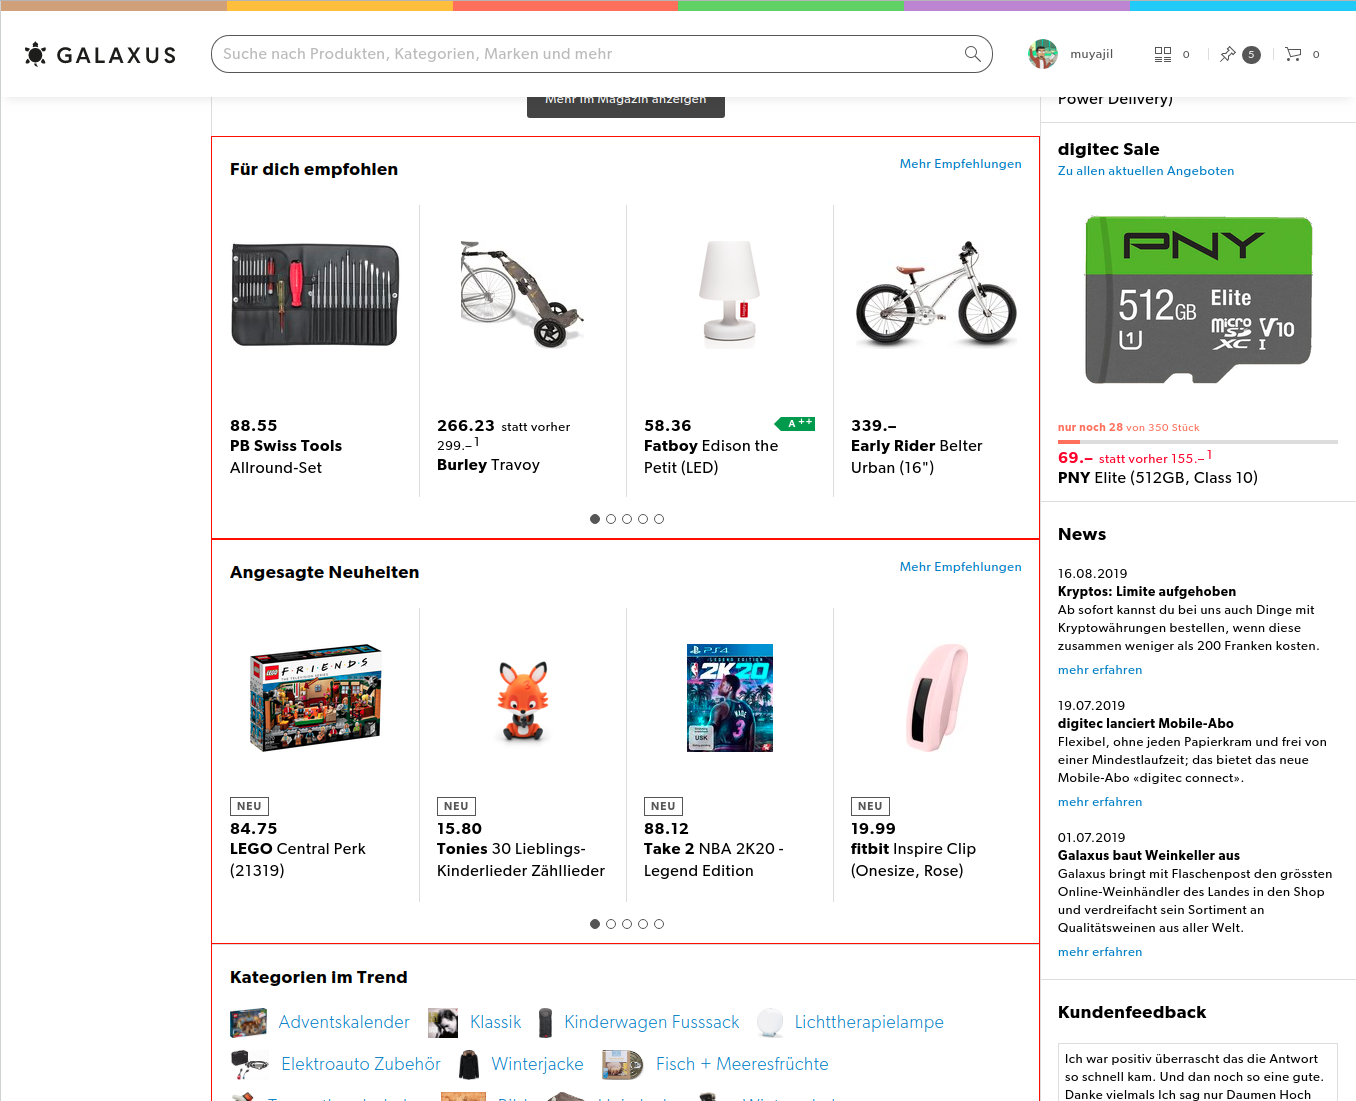
\includegraphics[width=\textwidth]{homepage-recs.png}
    \caption{Recommendations on the homepage}
    \label{fig:homepage_recs}
\end{figure}

\begin{figure}[t]
	\centering
	\captionsetup{width=0.8\textwidth}
    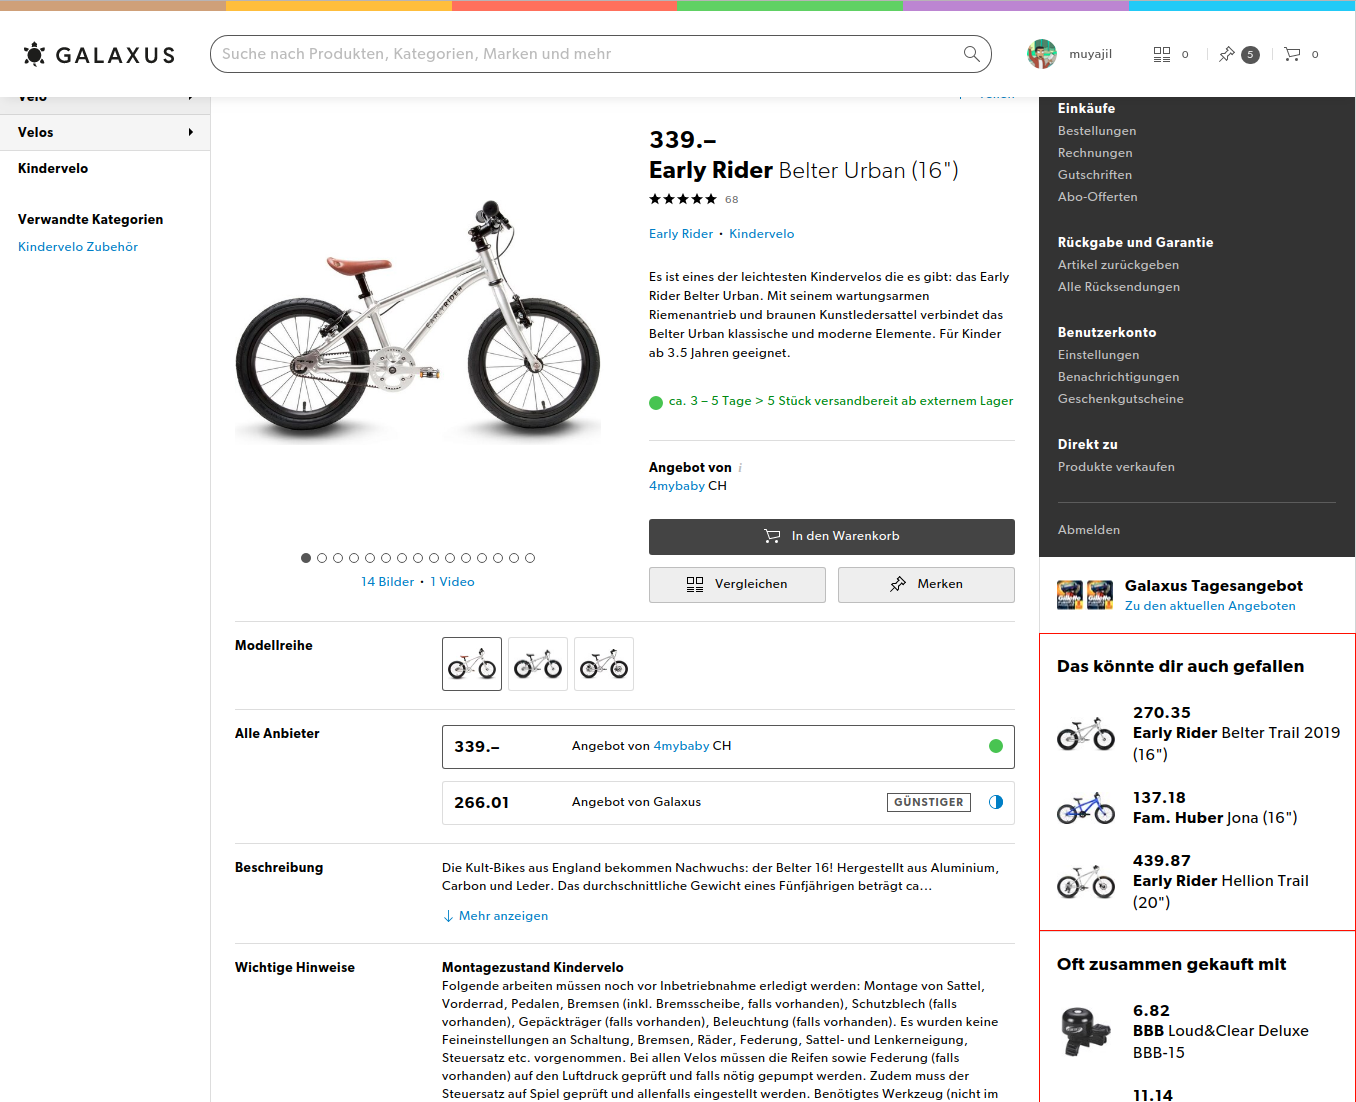
\includegraphics[width=\textwidth]{product-detail-recs.png}
    \caption{Recommendations on the product detail page}
    \label{fig:product_detail_recs}
\end{figure}

There is a framework that computes probabilities which specific recommendation engine provides the content for a specific location.
Further the framework then chooses the content for each location based on the probabilities computed before and some other constraints such as minimum and maximum value.
However to test the model implemented in this work this framework is bypassed by a A/B Testing engine, therefore this framework is not part of this work.
The specific tests and the test setup is described in~\ref{sec:exp_setup}, for the understanding of the following it is enough to assume that some independant system is providing recommendation requests to the recommendation system.
Using the API containers described in~\ref{sec:api} we can serve these requests.
The sequence-diagram in figure~\ref{fig:serving_recs} should give an overview on how the system is integrated in the production environment.

\begin{figure}[t]
	\centering
	\captionsetup{width=0.8\textwidth}
    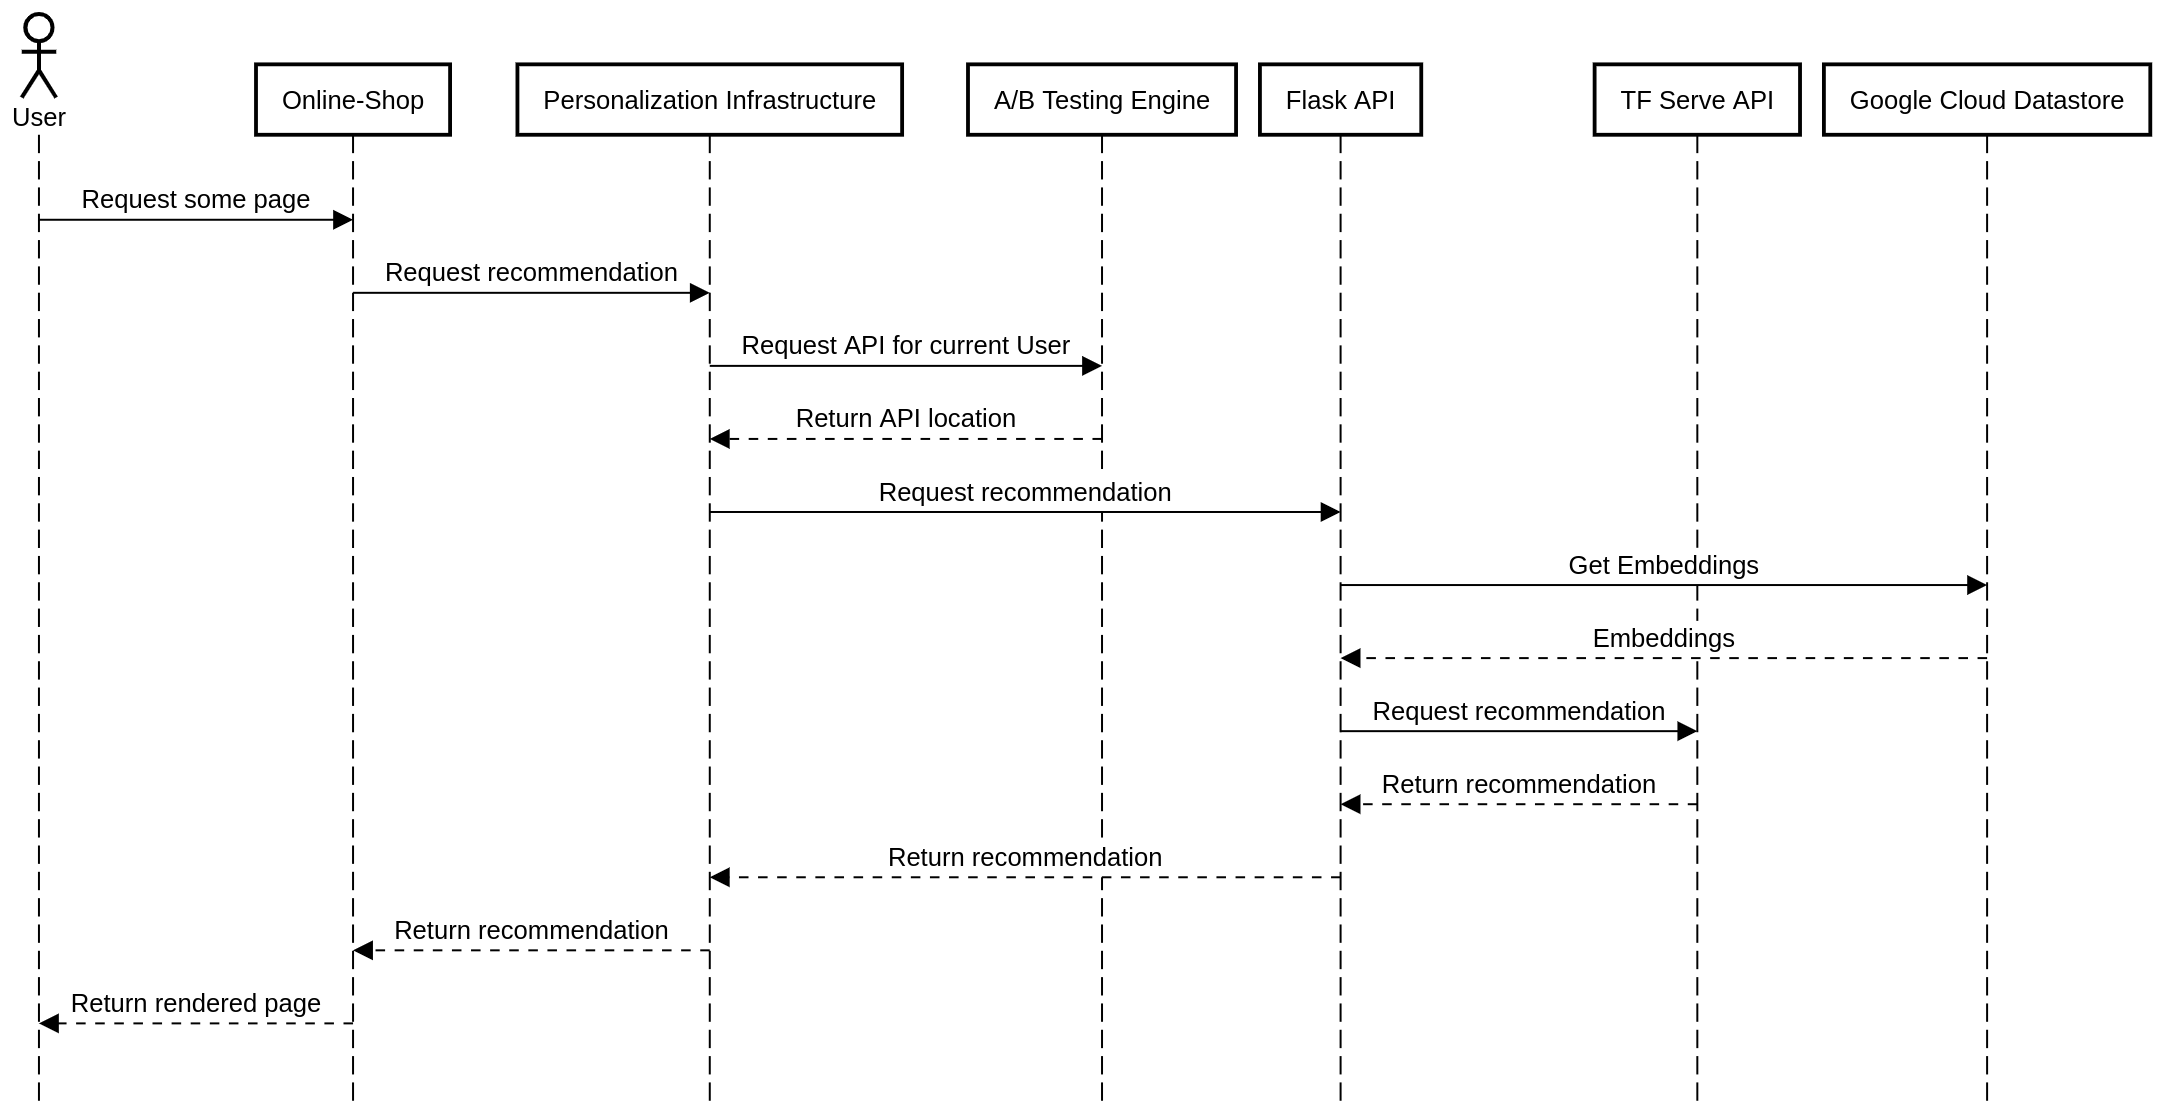
\includegraphics[width=\textwidth]{serving-recommendations.png}
    \caption{Serving Recommendations on digitec.ch and galaxus.ch}
    \label{fig:serving_recs}
\end{figure}

The whole process starts when a specific user requests a specific page on either digitec.ch or galaxus.ch.
If the requested page has an element where there is an A/B test configured the online shop Application will make a request to the testing engine.
The testing engine will return the API location of one of the model versions
After that the Online Shop will request the content, in this case, from the Personalization Infrastructure.
Note that during this setup each of the four versions of the model is deployed simultaneously, all of them trained on the same dataset.
The Personalization Infrastructure then calls the Middleware described above.
Before requesting a prediction from tf-serve the Middleware will gather precomputed embeddings for the involved entities.
The predictions are returned to the Personalization Infrastructure and from there to the Online Shop.
The last step is for the Online Shop to render the content and deliver the page to the user.
This process takes about 300ms.goal with this